\documentclass[]{article}
\newcommand{\FileDepth}{../../..}
\usepackage[letterpaper, landscape, margin=0.5cm]{geometry}
\usepackage[T1]{fontenc}
\usepackage{textcomp}%Not strictly necessary, but gives \textmu command for "micro."
\usepackage{fancyhdr}
\usepackage{amsmath}
\usepackage{amssymb}
\usepackage{graphicx}
\usepackage{xcolor}
\usepackage{tikz}
\usetikzlibrary{calc}
\usepackage[shortlabels]{enumitem}
\usepackage{multicol}
\usepackage{vwcol}
\usepackage{hyperref}
\usepackage{wrapfig}
%opening
\newcommand{\SecType}{L}
\newcommand{\Week}{23}
\title{PH 211 Lecture \Week}
\author{Benjamin Bauml}
\date{Summer 2024}

\newcommand{\Purpose}{4}
\newcommand{\DefOnly}{0}

% Version 2024-06-14
% Changes
% 2024-02-21 Added xstring package to enable smooth implementation of new \ModePage command.
% 2024-04-27 Set up to split activities and formatting aspects into separate files. Removed dependence on xcomment. Added an automatic counter to number the activities in a problem set.
% 2024-05-19 Revised old format for \TeachingTips command, which did not support \DefOnly.
% 2024-06-14 Added Repurpose environment to allow mixing of different purpose levels in the same document.
\usepackage{tcolorbox}
\usepackage{xstring}
% You will want the following four lines in your document (the last two uncommented):
% For Assignment, leave Purpose as 1. For Worksheet, set to 2. For Student Solution, set to 3. For Teacher Solution, set to 4.
% If you want keep the pieces from being called manually, set DefOnly to 0.
%\newcommand{\Purpose}{4}
%\newcommand{\DefOnly}{1}
\newcommand{\Exclusion}{0}
\newcommand{\PageTurn}{0}
\newcommand{\GrayProb}{0}
\newcommand{\Tipsy}{0}

% Assignment
\if\Purpose1
\renewcommand{\Exclusion}{1}
\fi
% Worksheet
\if\Purpose2
\renewcommand{\Exclusion}{1}
\renewcommand{\PageTurn}{1}
\fi
% Student Solution
\if\Purpose3
\renewcommand{\PageTurn}{1}
\renewcommand{\GrayProb}{1}
\fi
% Teaching Copy
\if\Purpose4
\renewcommand{\PageTurn}{1}
\renewcommand{\GrayProb}{1}
\renewcommand{\Tipsy}{1}
\fi

\newenvironment{Repurpose}[1]{
\renewcommand{\Purpose}{#1}
\renewcommand{\Exclusion}{0}
\renewcommand{\PageTurn}{0}
\renewcommand{\GrayProb}{0}
\renewcommand{\Tipsy}{0}
% Assignment
\if\Purpose1
\renewcommand{\Exclusion}{1}
\fi
% Worksheet
\if\Purpose2
\renewcommand{\Exclusion}{1}
\renewcommand{\PageTurn}{1}
\fi
% Student Solution
\if\Purpose3
\renewcommand{\PageTurn}{1}
\renewcommand{\GrayProb}{1}
\fi
% Teaching Copy
\if\Purpose4
\renewcommand{\PageTurn}{1}
\renewcommand{\GrayProb}{1}
\renewcommand{\Tipsy}{1}
\fi
}{}

\def \NewQ {0}
\def \PForce {0}
\newcommand{\MaybePage}[1]{
	\def \PForce {#1}
	\if\PForce1
	\newpage
	\else
	\if\NewQ0
	\gdef \NewQ {\PageTurn}
	\else
	\newpage
	\fi
	\fi
}

\newcommand{\ModePage}[1]{
	\IfSubStr{#1}{\Purpose}{\newpage}{}
}

\newcounter{ActNumber}
\setcounter{ActNumber}{0}

\newcommand{\Problem}[4][0]{%The first argument is optional, and if it is set to 1, the \newpage will be forced. The second argument is the name of the activity, the third is the command the activity is stored as, and the fourth is the actual problem statement.
\newcommand{#3}{
\MaybePage{#1}
\addtocounter{ActNumber}{1}
\section*{\SecType\Week-\theActNumber: #2}
\if\GrayProb1
\begin{tcolorbox}[colback=lightgray,colframe=lightgray,sharp corners,boxsep=1pt,left=0pt,right=0pt,top=0pt,bottom=0pt,after skip=2pt]
\else
\begin{tcolorbox}[colback=white,colframe=white,sharp corners,boxsep=1pt,left=0pt,right=0pt,top=0pt,bottom=0pt,after skip=2pt]
\fi
#4
\end{tcolorbox}\noindent
}
\if\DefOnly0
\else
#3
\fi
}
	
\newcommand{\ProblemSub}[3][0]{%The first argument is optional, and if a string of numbers is entered into it, it will force a \newpage in any \Purpose that shows up in the string. For example, "13" would lead to the newpage being forced in modes 1 and 3. The second is the command the activity is stored as, and the third is the actual problem statement.
\newcommand{#2}{
\ModePage{#1}
\if\GrayProb1
\begin{tcolorbox}[colback=lightgray,colframe=lightgray,sharp corners,boxsep=1pt,left=0pt,right=0pt,top=0pt,bottom=0pt,after skip=2pt]
\else
\begin{tcolorbox}[colback=white,colframe=white,sharp corners,boxsep=1pt,left=0pt,right=0pt,top=0pt,bottom=0pt,after skip=2pt]
\fi
#3
\end{tcolorbox}\noindent
}
\if\DefOnly0
\else
#2
\fi
}
		
\newcommand{\Solution}[2]{%The first argument is the command the solution is stored as, and the second is the actual solution.
\newcommand{#1}{
\if\Exclusion0
#2
\fi
}
\if\DefOnly0
\else
#1
\fi
}
		
\newcommand{\ProblemFig}[2]{%The first argument is the command the figure is stored as, and the second is the actual figure.
\newcommand{#1}{
\begin{figure}[h]
#2
\end{figure}
}
\if\DefOnly0
\else
#1
\fi
}

\newcommand{\TeachingTips}[2]{%The first argument is the command the tip is stored as, and the second is the actual tip.
\newcommand{#1}{
\if\Tipsy1
\begin{tcolorbox}[colback=lightgray,colframe=black]
#2
\end{tcolorbox}
\fi
}
\if\DefOnly0
\else
#1
\fi
}
\usepackage[absolute]{textpos}
% This package relies on Assignment Format 2024-06-14 or later to work. It is recommended that the Purpose and DefOnly commands be given as such:
%\newcommand{\Purpose}{4}
%\newcommand{\DefOnly}{0}
% Activities need to be entered outside of the TeacherMargin and PresentSpace environments, otherwise they will be defined only locally. They can even go in the preamble.
\newenvironment{TeacherMargin}{\begin{textblock*}{10.8cm}(0.5cm,0.5cm)
\small}{\end{textblock*}
\hspace{0.1cm}}
\newenvironment{PresentSpace}{\begin{textblock*}{0.3cm}(26.85cm,9.35cm)
--
\end{textblock*}
\begin{textblock*}{0.3cm}(26.85cm,18.7cm)
--
\end{textblock*}
\begin{textblock*}{0.3cm}(26.85cm,12.24cm)
	--
\end{textblock*}
\begin{textblock*}{15.6cm}(11.8cm,0.5cm)
\begin{Repurpose}{1}
\Large}{\end{Repurpose}
\end{textblock*}
\hspace{0.1cm}}

%\newcommand{\FBDaxes}[3]{
	\begin{scope}[shift={(#1)},rotate=#2]
		% x-axis
		\draw[thick,->] (-2,0) -- (2,0);
		\node[anchor=west] at (2,0) {$x$};
		% y-axis
		\draw[thick,->] (0,-2) -- (0,2);
		\node[anchor=west] at (0,2) {$y$};
		\coordinate (#3) at (0,0);
	\end{scope}
}
\newcommand{\FBDvectorMA}[4]{
	\begin{scope}[shift={(#1)}]
		\coordinate (#4tip) at ({#2*cos(#3)},{#2*sin(#3)});
		\draw[ultra thick,blue,->] (#1) -- (#4tip);
	\end{scope}
}
\newcommand{\FBDvectorXY}[3]{
	\begin{scope}[shift={(#1)}]
		\coordinate (#3tip) at (#2);
		\draw[ultra thick,blue,->] (0,0) -- (#3tip);
	\end{scope}
}
\newcommand{\FBDdot}[1]{
	\filldraw[black] (#1) circle (3pt);
}
%\newcommand{\MVec}[3][0]{%Creates a momentum vector of length #3 centered at #2 and rotated #1 degrees counterclockwise.
	\begin{scope}[rotate=#1,shift={(#2)}]
		\draw[->,thick] ({-#3/2},0) -- ({#3/2},0);
	\end{scope}
}
\newcommand{\MDot}[1]{%Creates a dot at #1 to represent a zero vector.
	\filldraw (#1) circle (1pt);
}
\newcommand{\MVDRows}[2][4.5]{%Creates the rows (initial, delta, final) of a momentum vector diagram. The optional argument determines the width of the table, and defaults to a good length for three columns (two objects and the total system). The non-optional argument gives a coordinate name (not displayed) to the diagram.
	\begin{scope}
		%\draw[thick] (0,5.5) -- (0,0);
		\draw[thick] (-1,4.5) -- (#1,4.5);
		\node at (-0.5,3.75) {$\vec{p}_{i}$};
		\draw[thick] (-1,3) -- (#1,3);
		\node at (-0.5,2.25) {$\Delta\vec{p}$};
		\draw[thick] (-1,1.5) -- (#1,1.5);
		\node at (-0.5,0.75) {$\vec{p}_{f}$};
		\coordinate (#2) at (0,5);
	\end{scope}
}
\newcommand{\MVDCol}[4][0.75]{%Creates a column for an object in a momentum vector diagram. The first (non-optional) argument is the coordinate name (not displayed) of the column, while the second is the displayed column header. The first argument also names the three entries down the column. The third argument anchors the column, so it should either be the coordinate name of the MVD (for the first column) or the coordinate name of the previous column. The optional argument indicates how far the center of the column should be from the previous column's edge, and defaults to 0.75
	\begin{scope}[shift={(#4)}]
		\node at (#1,0) {#3};
		%\draw[thick] ({#1*2},0.5) -- ({#1*2},-5);
		\draw[thick] (0,0.5) -- (0,-5);
		\coordinate (#2init) at (#1,-1.25);
		\coordinate (#2delt) at (#1,-2.75);
		\coordinate (#2fin) at (#1,-4.25);
		\coordinate (#2) at ({#1*2},0);
	\end{scope}
}

%\input{\FileDepth/Activities/Activity_One/Activity_One.tex}
%\input{\FileDepth/Activities/Activity_Two/Activity_Two.tex}

\begin{document}
\begin{TeacherMargin}

\end{TeacherMargin}
\begin{PresentSpace}
\begin{center}
	\huge Lecture \Week: Combining Physics Concepts II
\end{center}
\vspace{0.5cm}
\underline{Warm-Up Activity} \\
Question?
%\begin{multicols}{2}
\begin{enumerate}[(A)]
	\item Answer?
\end{enumerate}
%\end{multicols}
\end{PresentSpace}
\newpage
\begin{TeacherMargin}
\noindent $\vec{F}^{net}=\vec{0}$ in I and III, where the surface is flat. \\
$\vec{F}^{net}$ is down the ramp in II, and it doesn't matter which way the ball is moving, so it is the same for both motions.
\begin{center}
	\begin{tikzpicture}
		\node at (0,0) {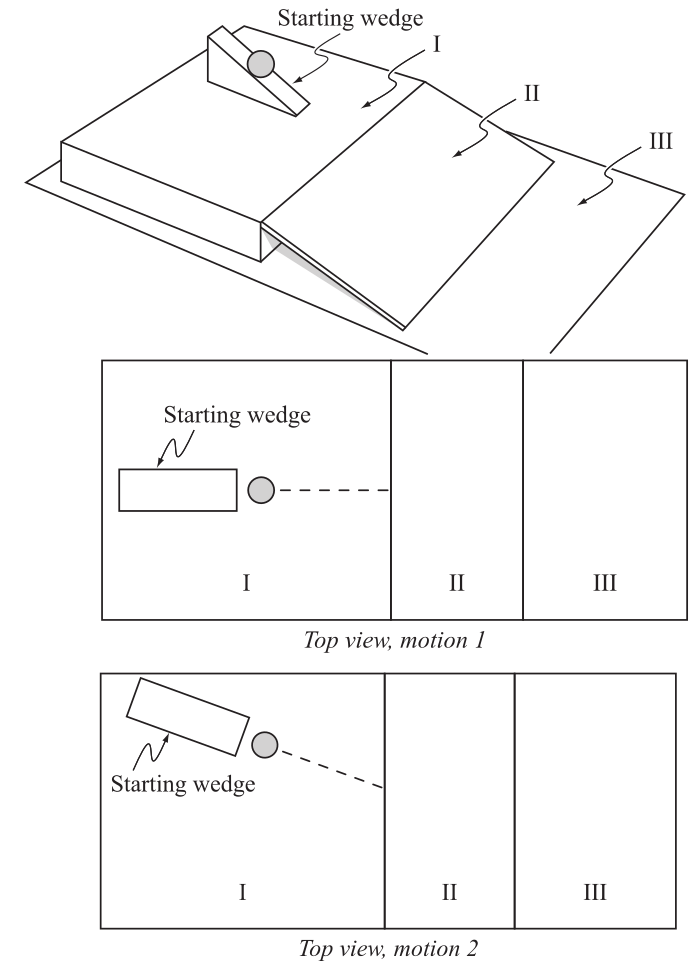
\includegraphics[scale=0.25]{WedgeRamp.png}};
		\draw[thick,->] (-0.5,2.3) -- (0,1.925) node[anchor=south west] {$\vec{F}^{net}$} -- (0.5,1.55);
		\draw[thick,violet] (-0.6,-0.06) -- (3,-0.06);
		\draw[ultra thick,blue,->] (-0.5,-0.5) node[anchor=east] {$\vec{p}_{i}$} -- (0.2,-0.5);
		\draw[ultra thick,blue,->] (1,-0.5) node[anchor=east] {$\Delta\vec{p}$} -- (1.5,-0.5);
		\draw[ultra thick,blue,->] (1.7,-0.5) node[anchor=north west] {$\vec{p}_{f}$} -- (3,-0.5);
		\draw[thick,violet] (-0.6,-2.35) -- (0.35,-2.7) .. controls (0.7,-2.8) .. (1.5,-3) -- (2.9,-3.265);
		\draw[dashed,violet] (0.35,-2.7) -- (1.5,-3.12);
		\draw[ultra thick,blue,->,shift={(-0.6,-2.5)},rotate=-20.225] (0,0) node[anchor=north] {$\vec{p}_{i}$} -- (0.7,0);
		\draw[ultra thick,blue,->,shift={(1.6,-3.2)},rotate=-10.728] (0,0) node[anchor=north west] {$\vec{p}_{f}$} -- (1.3,0);
		%\draw[ultra thick,blue,->,shift={(1.6,-3.2)},rotate=-20.225] (0,0) node[anchor=north] {$\vec{p}_{i}$} -- (0.7,0);
		%\draw[ultra thick,blue,->,shift={({1.6+0.7*cos(20.225)},{-3.2-0.7*sin(20.225)})}] (0,0) node[anchor=north] {$\Delta\vec{p}$} -- (0.6,0);
		\draw[ultra thick,blue,->,shift={(0.7,-2.3)}] (0,0) node[anchor=north] {$\Delta\vec{p}$} -- (0.6,0);
		\node[violet] at (-0.2,-1.9) {\tiny linear};
		\node[violet] at (0.95,-1.9) {\tiny parabolic};
		\node[violet] at (2.25,-1.9) {\tiny linear};
	\end{tikzpicture}
\end{center}
Trajectories are given in {\color{violet}violet}. Momenta are given in {\color{blue}blue}. As a side note, we can see just from this that $p_{i,y}=p_{f,y}$, as $\Delta\vec{p}$ is only in the $x$-direction. \\

\noindent Though the forces are the same, the ball in 2 spends more time on the ramp (it had less of its initial speed pointing straight down the ramp), so it gets more impulse. As such, its change in momentum is larger in magnitude than that of the ball in 1, but both are in the same direction, as the impulse is in the direction of the net force. \\
Conceptually, the change in momentum in 2 must be larger than the change in momentum in 1, as the momentum change in 2 not only increases the magnitude of the momentum (by the same amount as in 1, since the final momenta are the same; see below), but also must change its direction. This is the reverse triangle inequality:
\begin{center}
	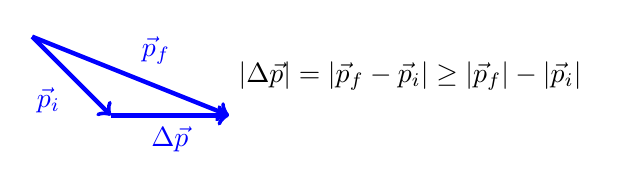
\begin{tikzpicture}
		\draw[ultra thick,blue,->] (0,0) -- (0.5,-0.5) node[anchor=north east] {$\vec{p}_{i}$} -- (1,-1);
		\draw[ultra thick,blue,->] (1,-1) -- (1.75,-1) node[anchor=north] {$\Delta\vec{p}$} -- (2.5,-1);
		\draw[ultra thick,blue,->] (0,0) -- (1.25,-0.5) node[anchor=south west] {$\vec{p}_{f}$} -- (2.5,-1);
		\node[anchor=west] at (2.5,-0.5) {$|\Delta\vec{p}| = |\vec{p}_{f}-\vec{p}_{i}| \geq |\vec{p}_{f}| - |\vec{p}_{i}|$};
	\end{tikzpicture}
\end{center}
\vspace{-10pt}
Regarding energy, if we look at this from a conservation of energy perspective, then the ball descends the same height in both motions, so $\Delta U_{g}$ is the same, and thus $\Delta K_{1} = \Delta K_{2}$. Thus, the balls' final speeds (and magnitudes of final momenta) must be the same. \\
From a work perspective, the work done on the ball in motion 1 is just $W_{1} = F\Delta x$, the force down the ramp times the displacement down the ramp. In motion 2, the displacement along the parabolic path is longer, but not in line with the force, so the dot product in $W_{2}=\int\vec{F}\cdot d\vec{x}$ will only keep the parts of the path in line with the force, giving us $W_{1}=W_{2}$.
\end{TeacherMargin}
\begin{PresentSpace}
\vspace{-10pt}
\section*{L\Week-1: Rolling a Ball}
\vspace{-10pt}
\begin{itemize}
	\large
	\item Sketch the trajectory of the ball in each case.
	\item Which ball spends more time in region II?
	\item How does the direction of the net force on \\
	the ball in motion 2 compare to the direction \\
	of the net force on the ball in motion 1?
	\item How does the change in kinetic energy of \\
	the ball in motion 1 compare to the change in \\
	kinetic energy of the ball in motion 2?
	\begin{itemize}
		\normalsize
		\item Is your answer consistent with the net work \\
		done on the ball in motions 1 and 2?
		\item How does the final speed of the ball in motion \\
		1 compare to the final speed in motion 2?
	\end{itemize}
	\item Draw vectors that represent the momentum \\
	of the ball at the top of the ramp and at the \\
	bottom of the ramp in each case.
	\begin{itemize}
		\normalsize
		\item How is the direction of the change in momentum \\
		related to the direction of the net force on the ball as it rolls down the ramp?
		\item How do the magnitudes of the changes in momentum in the two cases compare to each other?
	\end{itemize}
\end{itemize}
\end{PresentSpace}
\begin{textblock*}{5cm}(21cm,1.4cm)
\begin{center}
	\href{https://www.youtube.com/watch?v=3CjpPxNVjvA}{\tiny https://www.youtube.com/watch?v=3CjpPxNVjvA}
	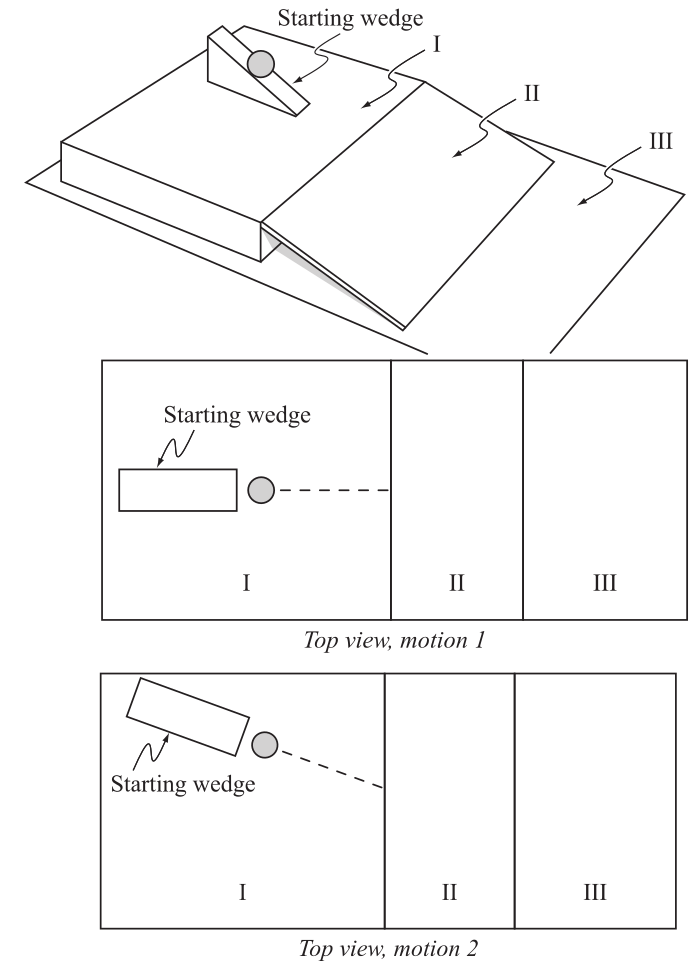
\includegraphics[scale=0.25]{WedgeRamp.png}
\end{center}
\end{textblock*}
\newpage
\begin{TeacherMargin}
\begin{center}
	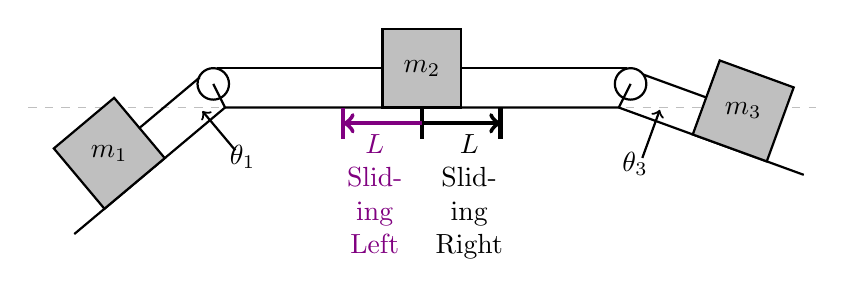
\begin{tikzpicture}
		\draw[lightgray,dashed] (0,0) -- (10,0);
		\draw[thick] (2.35,0.3) -- (2.5,0) -- (7.5,0) -- (7.65,0.3);
		\draw[thick] (2.4,0.5) -- (7.6,0.5);
		\draw[thick,color=black,fill=lightgray] (4.5,0) rectangle (5.5,1);
		\node at (5,0.5) {$m_{2}$};
		\draw[ultra thick] (5,0) -- (5,-0.4);
		\draw[ultra thick,->,violet] (5,-0.2) -- (4.4,-0.2) node[anchor=north] {\parbox{1cm}{\centering$L$ Sliding Left}} -- (4,-0.2);
		\draw[ultra thick,violet] (4,0) -- (4,-0.4);
		\draw[ultra thick,->] (5,-0.2) -- (5.6,-0.2) node[anchor=north] {\parbox{1cm}{\centering$L$ Sliding Right}} -- (6,-0.2);
		\draw[ultra thick] (6,0) -- (6,-0.4);
		\draw[thick] (2.35,0.3) circle (0.2);
		\draw[thick] (7.65,0.3) circle (0.2);
		\begin{scope}[shift={(2.5,0)},rotate=40]
			\draw[thick] (-2.5,0) -- (0,0);
			\draw[thick,color=black,fill=lightgray] (-2,0) rectangle (-1,1);
			\node at (-1.5,0.5) {$m_{1}$};
			\draw[thick] (-1,0.5) -- (0,0.5);
			\draw[thick,<-] (-0.25,0.15) -- (-0.25,-0.5) node[anchor=north west,shift={(-0.2,0.2)}] {$\theta_{1}$};
		\end{scope}
		\begin{scope}[shift={(7.5,0)},rotate=-20]
			\draw[thick] (0,0) -- (2.5,0);
			\draw[thick] (1,0.5) -- (0.15,0.5);
			\draw[thick,color=black,fill=lightgray] (1,0) rectangle (2,1);
			\node at (1.5,0.5) {$m_{3}$};
			\draw[thick,<-] (0.5,0.15) -- (0.5,-0.5) node[anchor=north east,shift={(0.2,0.2)}] {$\theta_{3}$};
		\end{scope}
	\end{tikzpicture}
\end{center}
If we wanted to know about acceleration, forces would make sense, but we just want to know about speed after the objects have moved some distance. We would need to do kinematics to get the final speed. Energy will be more direct, as it works with speed and position directly. \\

\noindent I will do the calculation assuming the boxes slide to the right, {\color{violet}but I will mark all changes for sliding left in violet.} \\
\newcommand{\Vpm}{
\begin{tikzpicture}
	\node[violet] at (0,0) {$+$};
	\node at (0,-0.1) {$-$};
\end{tikzpicture}
}
\newcommand{\Vmp}{
	\begin{tikzpicture}
		\node at (0,0) {$+$};
		\node[violet] at (0,0.1) {$-$};
	\end{tikzpicture}
}

\noindent Conservation of Energy: $0 = \Delta E_{\text{total}} = \Delta K + \Delta U_{g1} + \Delta U_{g2}$ \\
$\Delta K = K_{f}-K_{i} = K_{f} = \frac{1}{2}(m_{1}+m_{2}+m_{3})v^{2}$ \\
$\Delta U_{g1} = {\color{violet}-}m_{1}gL\sin\theta_{1}$ \quad Box 1 rises {\color{violet}(lowers)} by $h={\color{violet}-}L\sin\theta_{1}$. \\
$\Delta U_{g1} = \Vpm m_{1}gL\sin\theta_{3}$ \quad Box 3 lowers {\color{violet}(rises)} by $h={\color{violet}+}/-L\sin\theta_{3}$. \\
Our conservation of energy equation becomes
\[
\frac{1}{2}(m_{1}+m_{2}+m_{3})v^{2} {\color{violet}-}/+ m_{1}gL\sin\theta_{1} {\color{violet}+}/- m_{3}gL\sin\theta_{3} = 0,
\]
and therefore
\[
v=\sqrt{\frac{{\color{violet}-}2m_{3}gL\sin\theta_{3} {\color{violet}+}/-2m_{1}gL\sin\theta_{1}}{m_{1}+m_{2}+m_{3}}}
\]
\end{TeacherMargin}
\begin{PresentSpace}
\vspace{-10pt}
\section*{L\Week-2: Angled Ramps}
\vspace{-10pt}
\begin{center}
	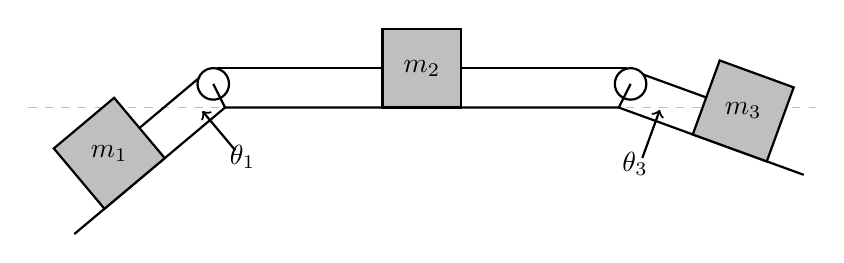
\begin{tikzpicture}
		\draw[lightgray,dashed] (0,0) -- (10,0);
		\draw[thick] (2.35,0.3) -- (2.5,0) -- (7.5,0) -- (7.65,0.3);
		\draw[thick] (2.4,0.5) -- (7.6,0.5);
		\draw[thick,color=black,fill=lightgray] (4.5,0) rectangle (5.5,1);
		\node at (5,0.5) {$m_{2}$};
		\draw[thick] (2.35,0.3) circle (0.2);
		\draw[thick] (7.65,0.3) circle (0.2);
		\begin{scope}[shift={(2.5,0)},rotate=40]
			\draw[thick] (-2.5,0) -- (0,0);
			\draw[thick,color=black,fill=lightgray] (-2,0) rectangle (-1,1);
			\node at (-1.5,0.5) {$m_{1}$};
			\draw[thick] (-1,0.5) -- (0,0.5);
			\draw[thick,<-] (-0.25,0.15) -- (-0.25,-0.5) node[anchor=north west,shift={(-0.2,0.2)}] {$\theta_{1}$};
		\end{scope}
		\begin{scope}[shift={(7.5,0)},rotate=-20]
			\draw[thick] (0,0) -- (2.5,0);
			\draw[thick] (1,0.5) -- (0.15,0.5);
			\draw[thick,color=black,fill=lightgray] (1,0) rectangle (2,1);
			\node at (1.5,0.5) {$m_{3}$};
			\draw[thick,<-] (0.5,0.15) -- (0.5,-0.5) node[anchor=north east,shift={(0.2,0.2)}] {$\theta_{3}$};
		\end{scope}
	\end{tikzpicture}
\end{center}
\begin{itemize}
	\large
	\item The three boxes shown at right are connected by ideal strings and pulleys. Assume the surface is frictionless. The boxes are initially at rest.
	\begin{itemize}
		\item Do you think this situation will be easier to analyze using \textbf{forces} or \textbf{energy}? Does your answer depend on what quantity you are looking for?
	\end{itemize}
	\item What is the speed of box 2 after it has moved a distance $L$?
	\begin{itemize}
		\item Evaluate your answer in at least 3 special cases.
		\item Is there any relationship between the three masses that will cause the blocks to remain at rest?
	\end{itemize}
\end{itemize}
\end{PresentSpace}
\newpage
\begin{TeacherMargin}
	
\end{TeacherMargin}
\begin{PresentSpace}
\section*{Main Ideas}
\begin{itemize}
	\item The work-energy and impulse-momentum theorems can be used to solve a broad array of problems.
\end{itemize}
\end{PresentSpace}
\end{document}